\section{Identifikation der Parameter}

Das im Theorieteil betrachtete Modell des Furuta-Pendels (siehe \citep{Cazzolato.2011}) unterscheidet sich von dem Modell des zu verwendenden Furuta-Pendels des Institutes, wie in Abb.~\ref{fig.parameter} 
ersichtlich.
Die gegeben bzw. gemessenen Parameter müssen daher an das theoretische Modell angepasst werden. Für die Längen der Pendelarme gilt somit:
\begin{eqnarray}
L_1 &=& l_a \nonumber \\
L_2 &=& l_{pm}

\end{eqnarray}

\begin{figure}[htbp]
	\centering	
	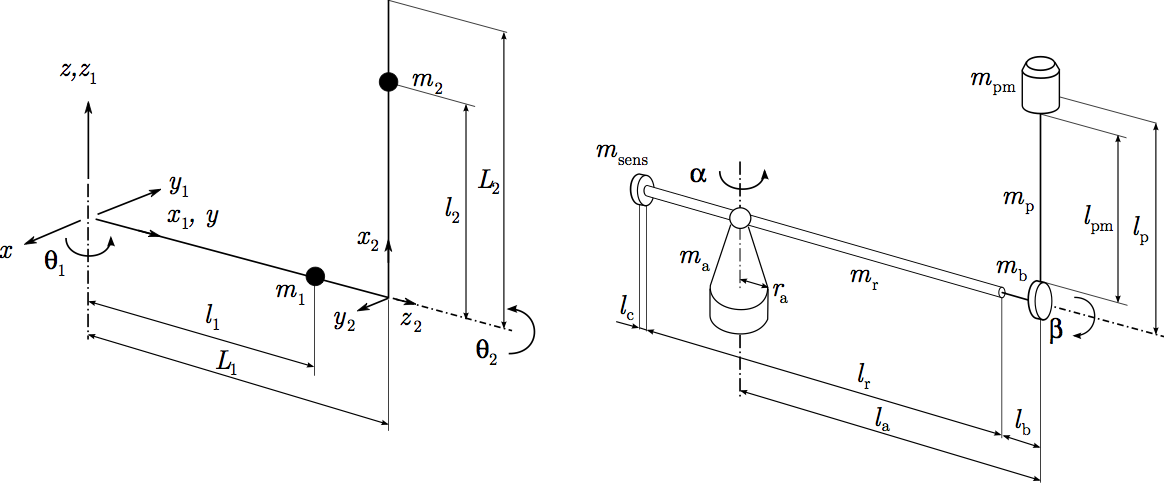
\includegraphics[width=1\textwidth]{Grafiken/ParameterFuruta.png}
	\caption{links: Modell der University of Adelaide, rechts das Set-Up der TUHH}
	\label{fig.parameter}
\end{figure}
l_sens=l_r+l_b-l_a+l_c/2;
Die Punktmassen des theoretischen Pendel-Modells ergeben sich bei Beachtung der Trägheitsachsen zu:
\begin{eqnarray}
m_1 &=& m_{sens}+m_r+m_a \nonumber \\
m_2 &=& m_p+m_{pm}
\end{eqnarray}
Die Massenträgheiten... %TODO
%Kai: ich habe einfach unsere equations aus matlab eingefügt!
\begin{eqnarray}
J_{1,norm}&=&\dfrac{J_M +J_{Enc1}+(m_r \cdot l_r \cdot l_r)}{12+(m_r (-0.5 l_r-l_b+l_a)^2)+(4/10) (m_a  {r_a}^{2})} \\
J_{2,norm}&=& J_{m,b}+J_{Enc2}   + \dfrac{(m_p \cdot {l_p}^{2})}{3} \\
J_0&=&J_{1,norm}+ m_1 \cdot {l_1}^{2} + m_2 \cdot {L_1}^{2} \\ 
J_2&=&J_{2,norm}+m2 \cdot {l_2}^2           \\
\end{eqnarray}
\begin{eqnarray}
l1=sqrt((l_sens.^2 \dot m_sens+l_b.^2 \dot m_b)./(m_sens+m_b));
l2=l_pm
\end{eqnarray}

%Kai: ab hier sind das wieder die von dustin/den anderen!
\begin{equation}
J_{arm} = m_r \frac{l^2_r}{12}+m_r(\frac{1}{2}l_r+l_b-l_a)^2
\end{equation}

\begin{equation}
J_{pend1}=m_bl^2_a
\end{equation}

\begin{equation}
J_{sens}=m_{sens}(l_a-l_b-l_r-\frac{1}{2}l_c)^2
\end{equation}

\begin{equation}
J_{ps}=m_p(r_b+\frac{1}{2}l_p)^2
\end{equation}

\begin{equation}
J_{pm}=m_{pm}l^2_{pm}
\end{equation}

\begin{equation}
J_{arm}+J_{pend1}+J_{sens}=m_1l^2_1J_{pm}+J_{ps}=m_2l^2_2
\end{equation}

%Hier sind unsere werte! noch viele Latex-Fehler!

\begin{eqnarray}
b1=1e-4 \\
b2=2.8e-4 \\
g=9.81\\
k_{1,phi}=0.5\\
R_a=10\\
J_M = 6.75e-6  \\        % Inertia Motor 6.75e-6
J_{Enc1} = 6e-14 \\        % Inertia Encoder Theta1
J_{Enc2} = 0.1e-6  \\     % Inertia Encoder Theta2
J_{m,b} = 3.98125e-6 \\     % Inertia m_b
m_{sens} = 0.084  \\
l_c = 0.01 \\
m_{horzArm}=0.284 \\
m_b=0.025 \\
m_a=.190 \\
r_a=.015 \\
r_b=\dfrac{0.0352}{2}\\
l_r=0.29\\
m_r = m_{horzArm} - m_{sens}\\
l_a=.175\\
l_b=.01\\
m_{pm}=0.0379\\
m_p=0.0157\\
l_{pm}=0.229\\
l_p=0.262\\
\end{eqnarray}


Die Gleichung des DC-Motors, der den Pendelarm und somit direkt $\theta_2$ antreibt, kann aus der gegebenen Formel des Research Articles der University of Adelaide, abgeleitet werden.\cite{Cazzolato.2011}
Auch die Parameter des DC-Motors wurden aus dem Dokument entnommen. Folgende Parameter sind gegeben:

\begin{eqnarray}
K_m &=& 0,09  \dfrac{Nm}{A} \\
R_m &=& 7,8  \Omega \\
L_m &=& 0,005  H \\
\end{eqnarray}